\documentclass[a4paper]{article}

\usepackage{fullpage} % Package to use full page
\usepackage{parskip} % Package to tweak paragraph skipping
\usepackage{tikz} % Package for drawing
\usepackage{amsmath}
\usepackage{hyperref}
\usepackage{pdfpages} % For inserting entire pages from a PDF
\usepackage{graphicx} % For including images

\title{Zero to Hero: WiMo}
\author{Niels Savvides}
\date{2024/10/30}

\begin{document}

\maketitle

\section{Analyse in 1 veranderlijke: enkele aspecten}

\subsection{Continuiteitseigenschappen van functies}

Functie $f(x)$ is contine over $]a,b[$ als:
\begin{enumerate}
	\item $f(x)$ bestaat in elk punt
	\item de limiet van $f(x)$ bestaat in elk punt
\end{enumerate}

\textbf{Continue afgeleide}: $f(x)$ is continue (zie hierboven) en $f'(x)$ bestaat in elk punt.
Dit kan:
\begin{enumerate}
	\item gladde functies zijn: elk afgeleide is continue
	\item stuksgewijs: $f(x)$ heeft een singulariteit, maar het bestaat in deel intervallen $]a, c[$ $]c, b[$
\end{enumerate}

\begin{figure}[!htbp]
	\begin{center}
		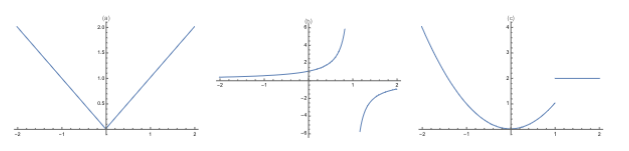
\includegraphics[width=8cm]{./images/continu.png}
	\end{center}
	\caption{a) Continue functie, stukgewijs continue afgeleide (als je afleid krijg je een singulareit) b) Heeft een singulaireit, dus stukgewijs continue, stukgewijs glad continue afleidbaar c) Deze is glad stukgewijs continue afleidbaar, is ook stukgewijs continue }
\end{figure}


\subsection{Taylorontwikkeling}
\label{sec:taylor}

We willen zaken gaan benaderen. Hiervoor gebruiken we:

$ f(x) = f(a) + f'(a)(x-a) + \frac{f''(a)}{2!}(x-a)^2 + \frac{f'''(a)}{3!}(x-a)^3 + ... $

waarbij $a$ het \textbf{werkpunt} is.

Veel voorkomende Taylorontwikkelingen:

See Figure \ref{fig:veel_voorkomend_taylor}.

\begin{figure}[htbp!]
	\centering
	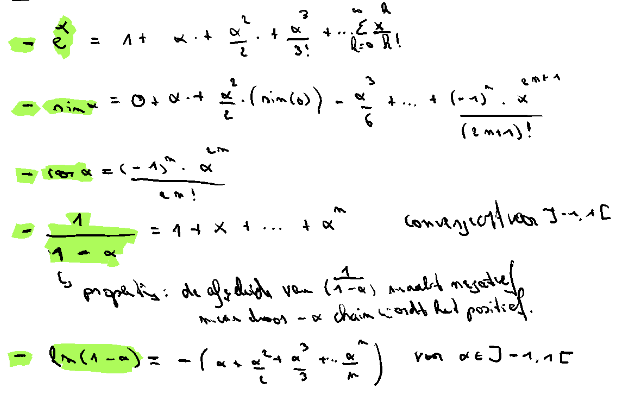
\includegraphics[width=0.8\textwidth]{assets/veel_voorkomend_taylor.png}
	\caption{Simply use the formulas}
	\label{fig:veel_voorkomend_taylor}
\end{figure}

\subsection*{Storingsrekening}

Zie Figuur \ref{fig:storing_solution}.

Of Maple solution \ref{sol:storing}.

\begin{figure}[!htbp]
	\centering
	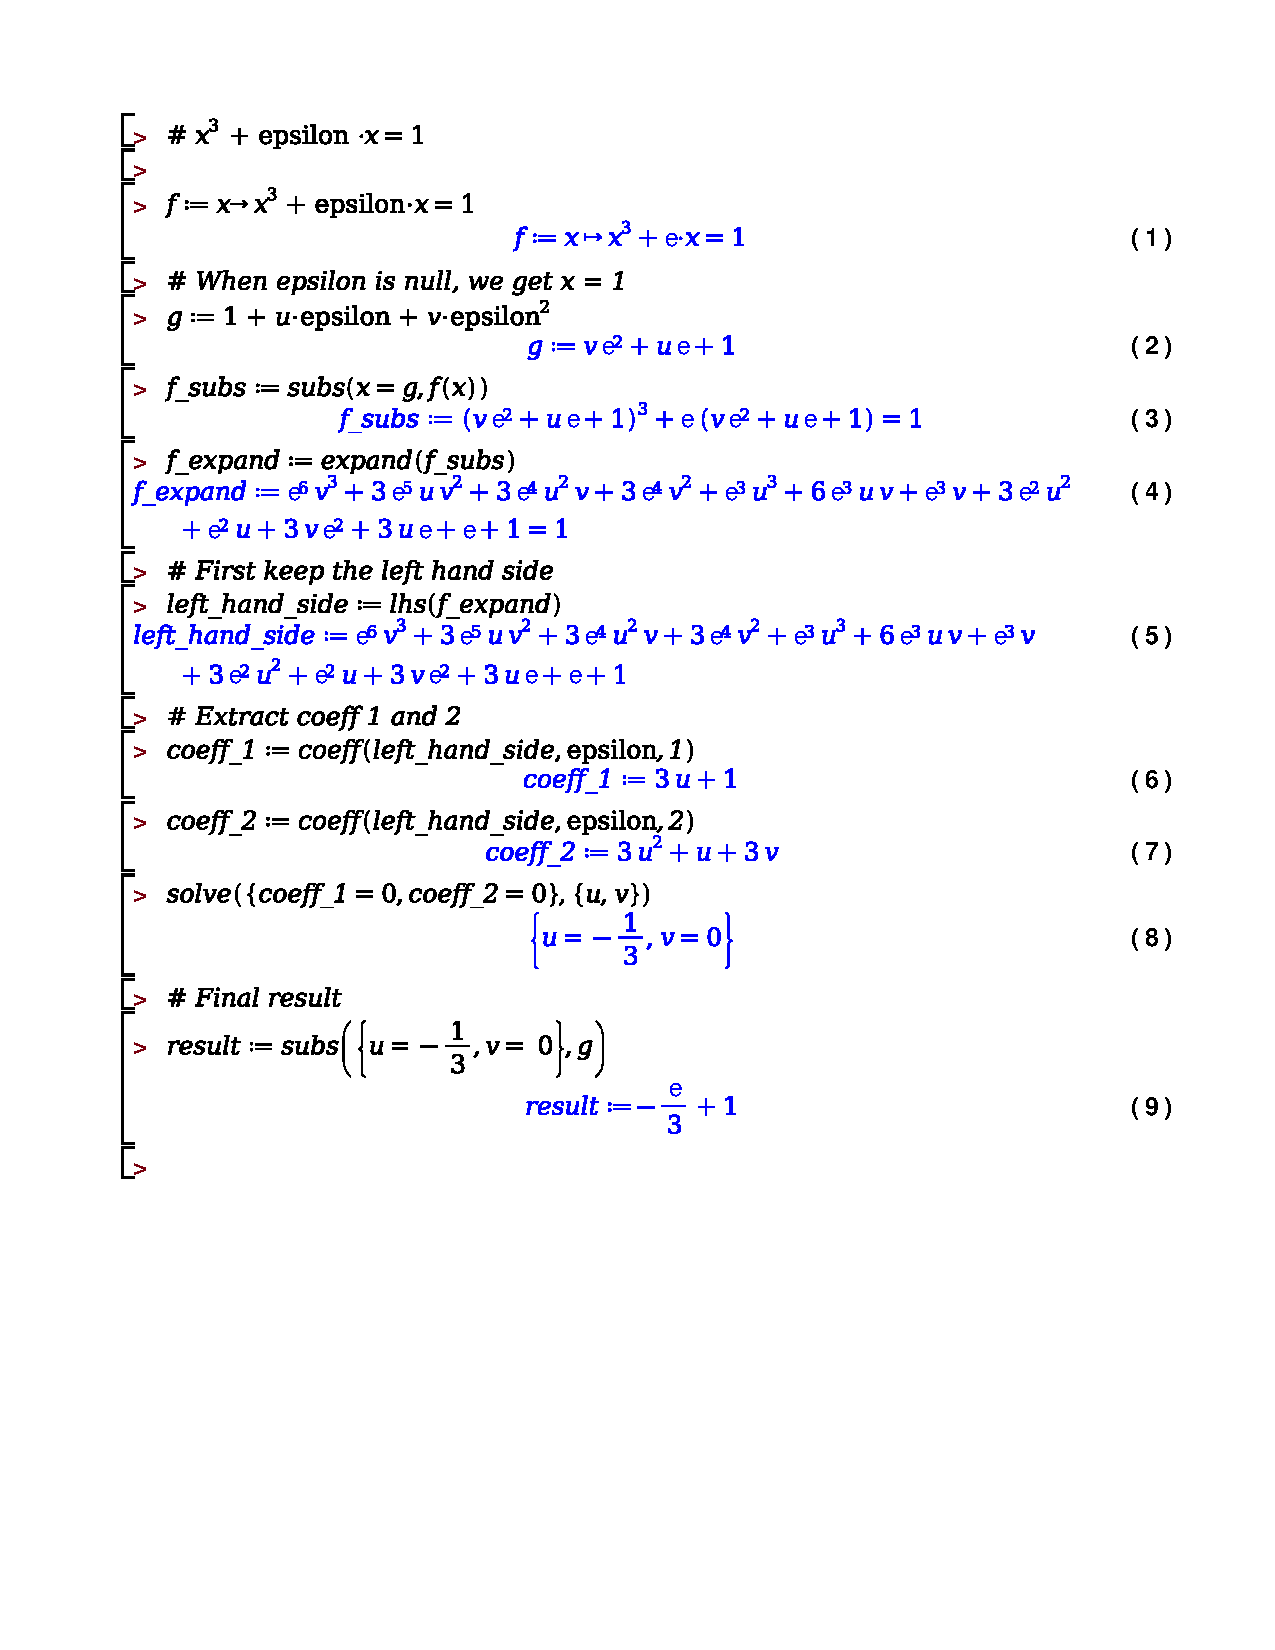
\includegraphics[width=\textwidth]{./storing.pdf}
	\caption{Maple solution}
	\label{sol:storing}
\end{figure}

\begin{figure}[htbp!]
	\centering
	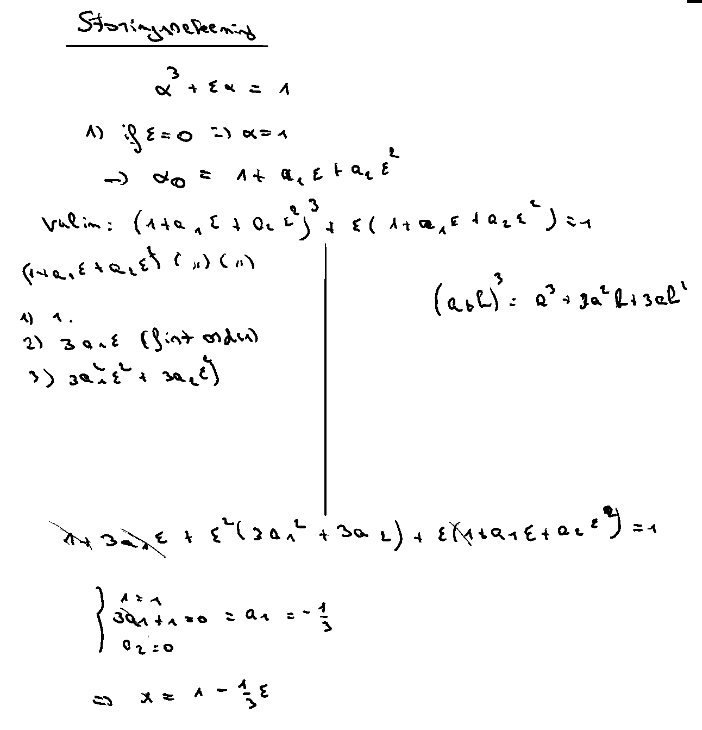
\includegraphics[width=0.8\textwidth]{assets/storing_solution.png}
	\caption{1. Merk op dat als epsilon 0 is, dan is x = 1. Dus we benaderen value 1: $1 + \epsilon . u + \epsilon^2 . v$. Vul dit in the main equation. Gebruik maple om dit op te lossen en vul $u$ en $v$ in $x_1$}
	\label{fig:storing_solution}
\end{figure}

\subsection{Twee eenvoudige differentiaalvergelijkingen}

\subsubsection{Eerste orde differentiaalvergelijking}

$y'(x) = \lambda y(x)$

Als we dit uitwerken krijgen we:

$ln(y(x)) = \lambda x + C$

$y(x) = e^{\lambda x + C} = e^C e^{\lambda x} = C e^{\lambda x}$ met $C = y(0)$

$y(x) = y(0) e^{\lambda x}$

\subsubsection*{Radioactief verval}

Zie Figuur \ref{fig:radio_solution}.

\begin{figure}[htbp!]
	\centering
	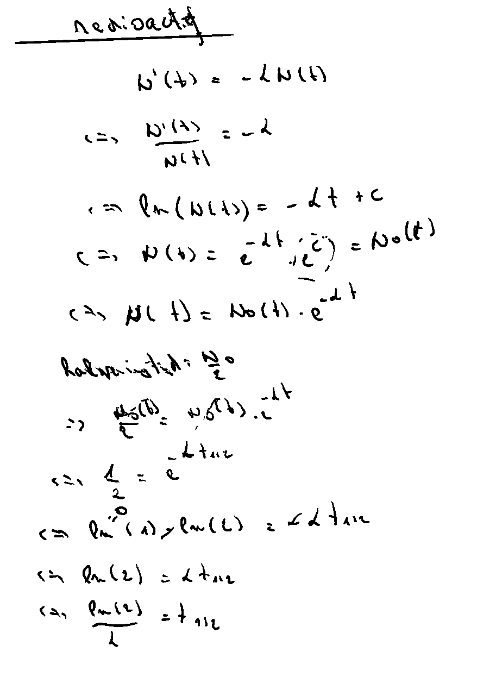
\includegraphics[width=0.8\textwidth]{assets/radio_solution.png}
	\caption{Vindt eerst de differentiaalvergelijking (zie eerste differentiaalvergelijking). Dan kunnen we de oplossing gelijkstellen aan $N_0 / 2$. Werk dit uit en je hebt $t_{1/2}$ gevonden}
	\label{fig:radio_solution}
\end{figure}

\subsubsection{Tweede orde differentiaalvergelijking}

$y''(x) = \lambda y(x)$

Hierbij heb je 3 gevallen:

1. $\lambda > 0$: $y(t) = A e^{\sqrt{\lambda} t} + B e^{-\sqrt{\lambda} t}$

2. $\lambda = 0$: $y(t) = A + Bt$

3. $\lambda < 0$: $y(t) = A cos(\sqrt{-\lambda} t) + B sin(\sqrt{-\lambda} t)$

\subsubsection{Complexe getallen}

Algemene vorm: $z = a + bi$

waarbij $a$ reeel, $b$ imaginair en $i^2 = -1$

\textbf{inverse}: $(a + bi)^{-1} = \frac{a - bi}{a^2 + b^2}$

\textbf{complement}: $z = a + bi \rightarrow z^* = a - bi$

\textbf{modulus}: $|z| = \sqrt{a^2 + b^2}$

in \textbf{polaire vorm}:

$e^{i\theta} = cos(\theta) + i sin(\theta)$ (Dit kan via Taylor bewezen worden (zie oefeningen))

Okey, nu nog een paar goniometrische formules:

$sin^2(x) + cos^2(x) = 1$

$sin(x) = \frac{e^{ix} - e^{-ix}}{2i}$

$sin(2x) = 2sin(x)cos(x)$

$cos(x) = \frac{e^{ix} + e^{-ix}}{2}$

$cos(2x) = cos^2(x) - sin^2(x)$

\subsubsection{Hoofdstelling van de algebra}

Als we een kwadratisch veelterm hebben: $ax^2 + bx + c = 0$

Dan vinden we de nulpunten (oplossingen) met:

$x_1 = \frac{-b + \sqrt{b^2 - 4ac}}{2a}$

$x_2 = \frac{-b - \sqrt{b^2 - 4ac}}{2a}$

met $b = -4*a*c$ vinden we de discriminant.


\section*{Formularium}

\subsection*{Taylorontwikkeling}

- $ f(x) = f(a) + f'(a)(x-a) + \frac{f''(a)}{2!}(x-a)^2 + \frac{f'''(a)}{3!}(x-a)^3 + ... $

- $sin(x) = x$ voor kleine $x$

\subsection*{Differentiaalvergelijkingen}

- $y'(x) = \lambda y(x)$

- $y''(x) = \lambda y(x)$ (hier werden 3 gevallen besproken)

\subsection*{Complexe getallen}

- $z = a + bi$ (algemene vorm)

- $i^2 = -1$

- \textbf{inverse}: $(a + bi)^{-1} = \frac{a - bi}{a^2 + b^2}$

- \textbf{complement}: $z = a + bi \rightarrow z^* = a - bi$

- \textbf{modulus}: $|z| = \sqrt{a^2 + b^2}$

- $e^{i\theta} = cos(\theta) + i sin(\theta)$

- $sin^2(x) + cos^2(x) = 1$

- $sin(x) = \frac{e^{ix} - e^{-ix}}{2i}$

- $sin(2x) = 2sin(x)cos(x)$

- $cos(x) = \frac{e^{ix} + e^{-ix}}{2}$

- $cos(2x) = cos^2(x) - sin^2(x)$

\subsection*{Hoofdstelling van de algebra}

$x_1 = \frac{-b + \sqrt{b^2 - 4ac}}{2a}$

$x_2 = \frac{-b - \sqrt{b^2 - 4ac}}{2a}$

met $b = -4*a*c$


\section*{Oefeningen}

\subsection*{Huis 1}

\begin{figure}[!htbp]
	\centering
	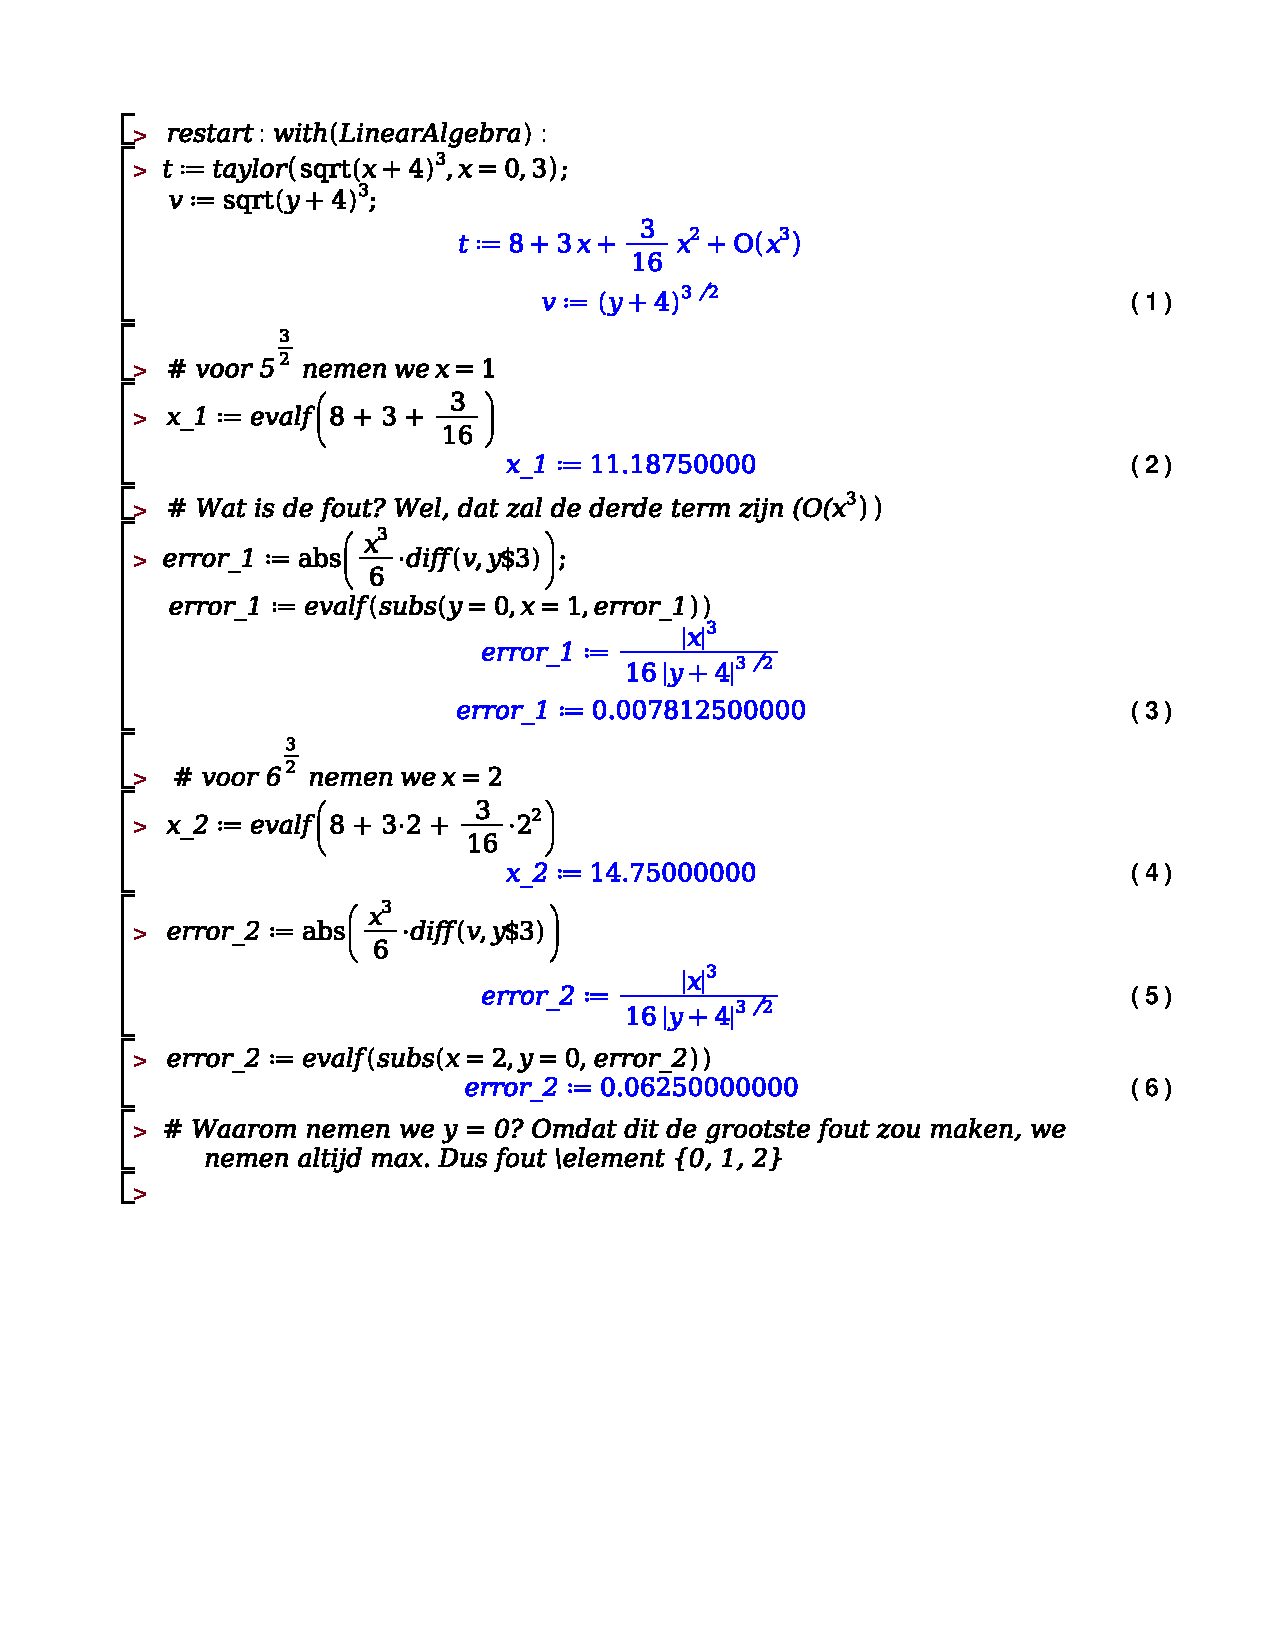
\includegraphics[width=0.8\textwidth]{./exercises/huis_1_ex_1.pdf}
	\caption{Exercise 1}
\end{figure}

\begin{figure}[!htbp]
	\centering
	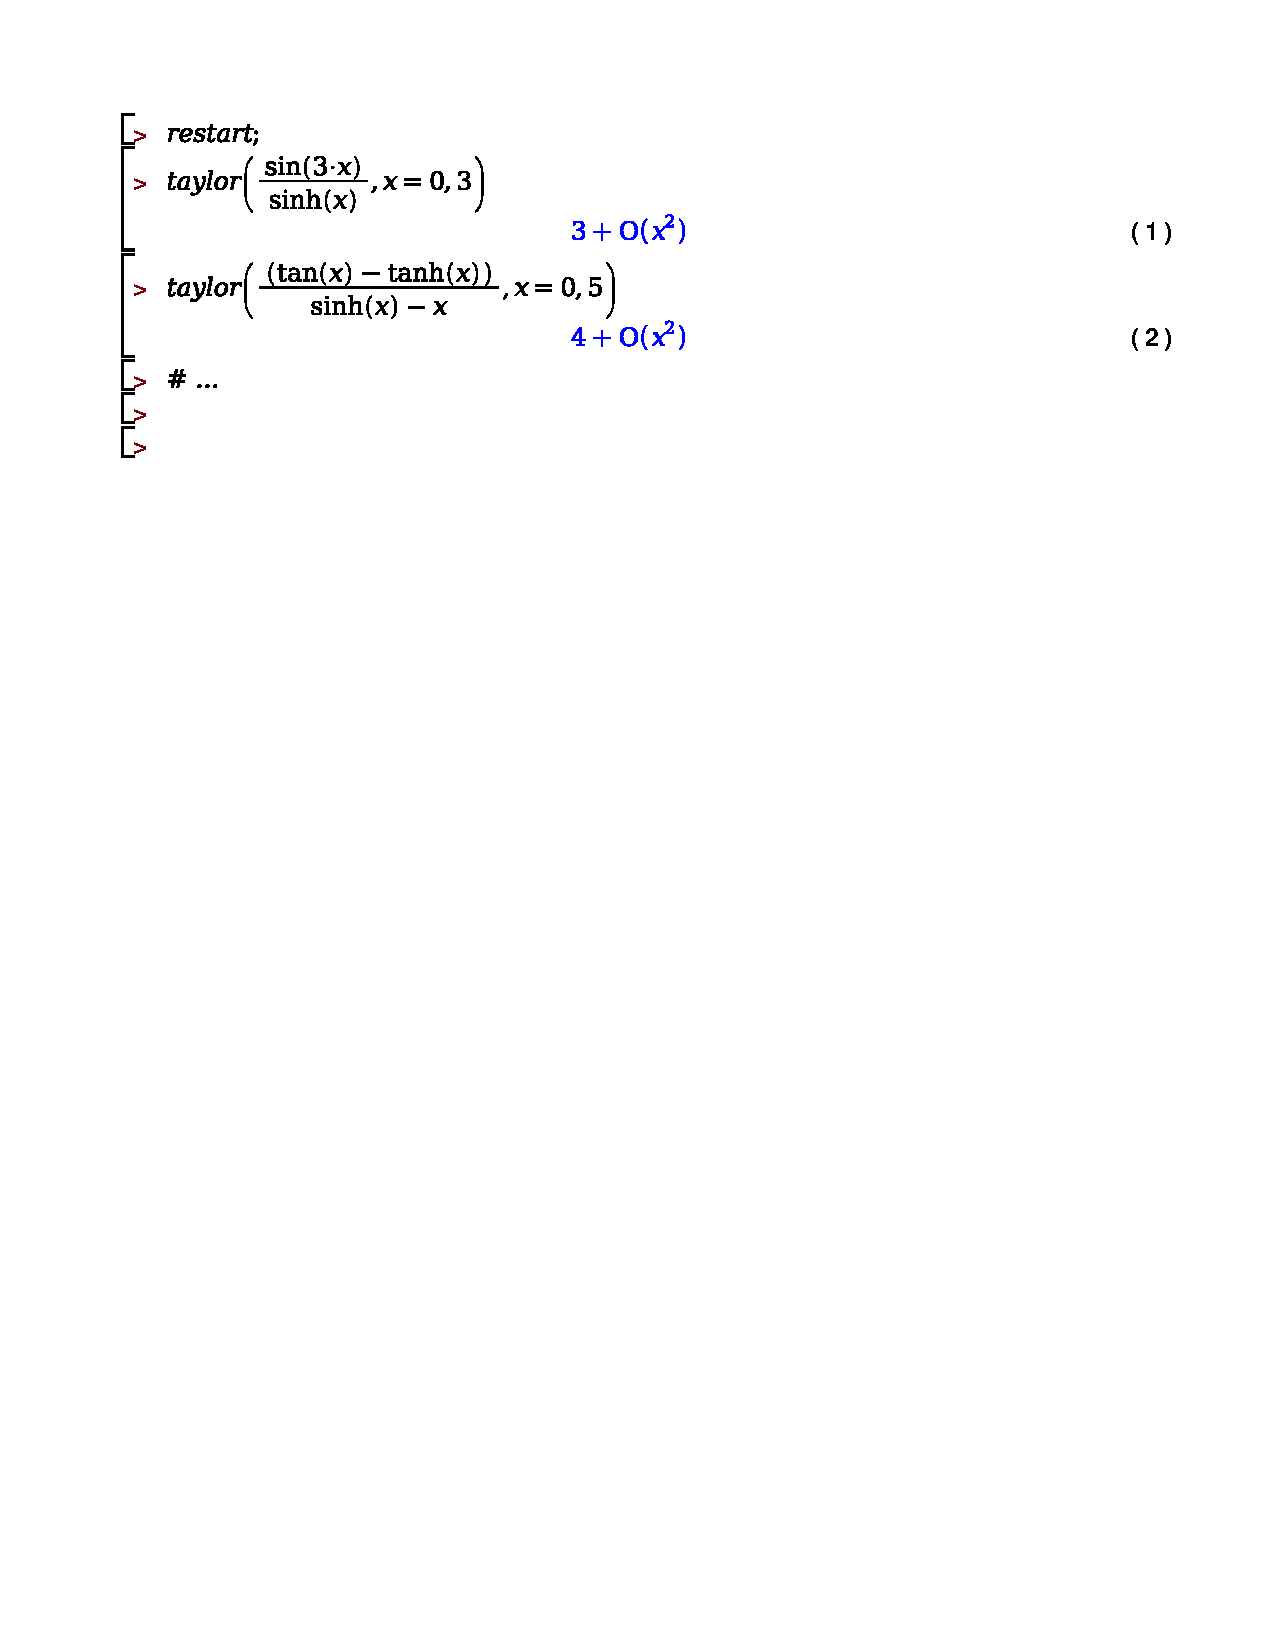
\includegraphics[width=0.8\textwidth]{./exercises/huis_1_ex_2.pdf}
	\caption{Exercise 2}
\end{figure}



\begin{figure}[!htbp]
	\centering
	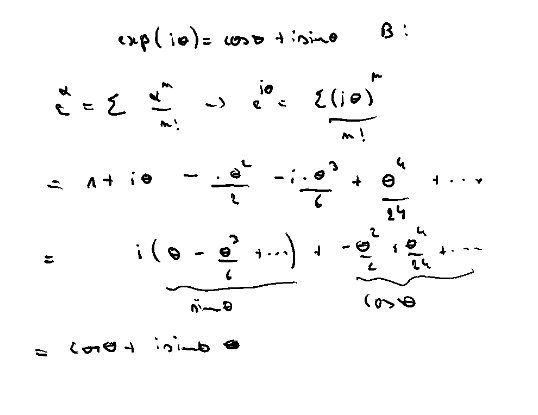
\includegraphics[width=0.8\textwidth]{assets/huis_1_ex_3.png}
	\caption{Exercise 3}
	\label{fig:huis_1_ex_3}
\end{figure}


\begin{figure}[!htbp]
	\centering
	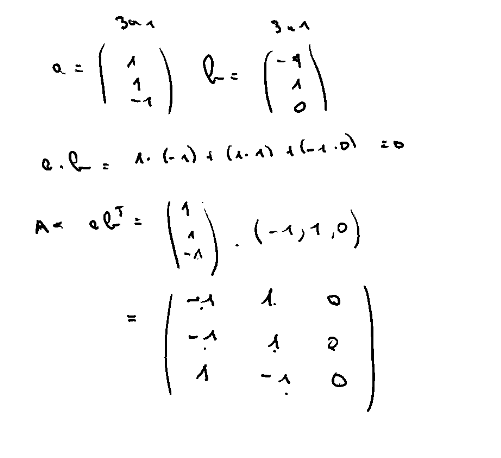
\includegraphics[width=0.6\textwidth]{assets/huis_1_ex_4.png}
	\caption{Exercise 4}
	\label{fig:huis_1_ex_4}
\end{figure}

\newpage

\subsection*{WC 1}

\begin{figure}[!htbp]
	\centering
	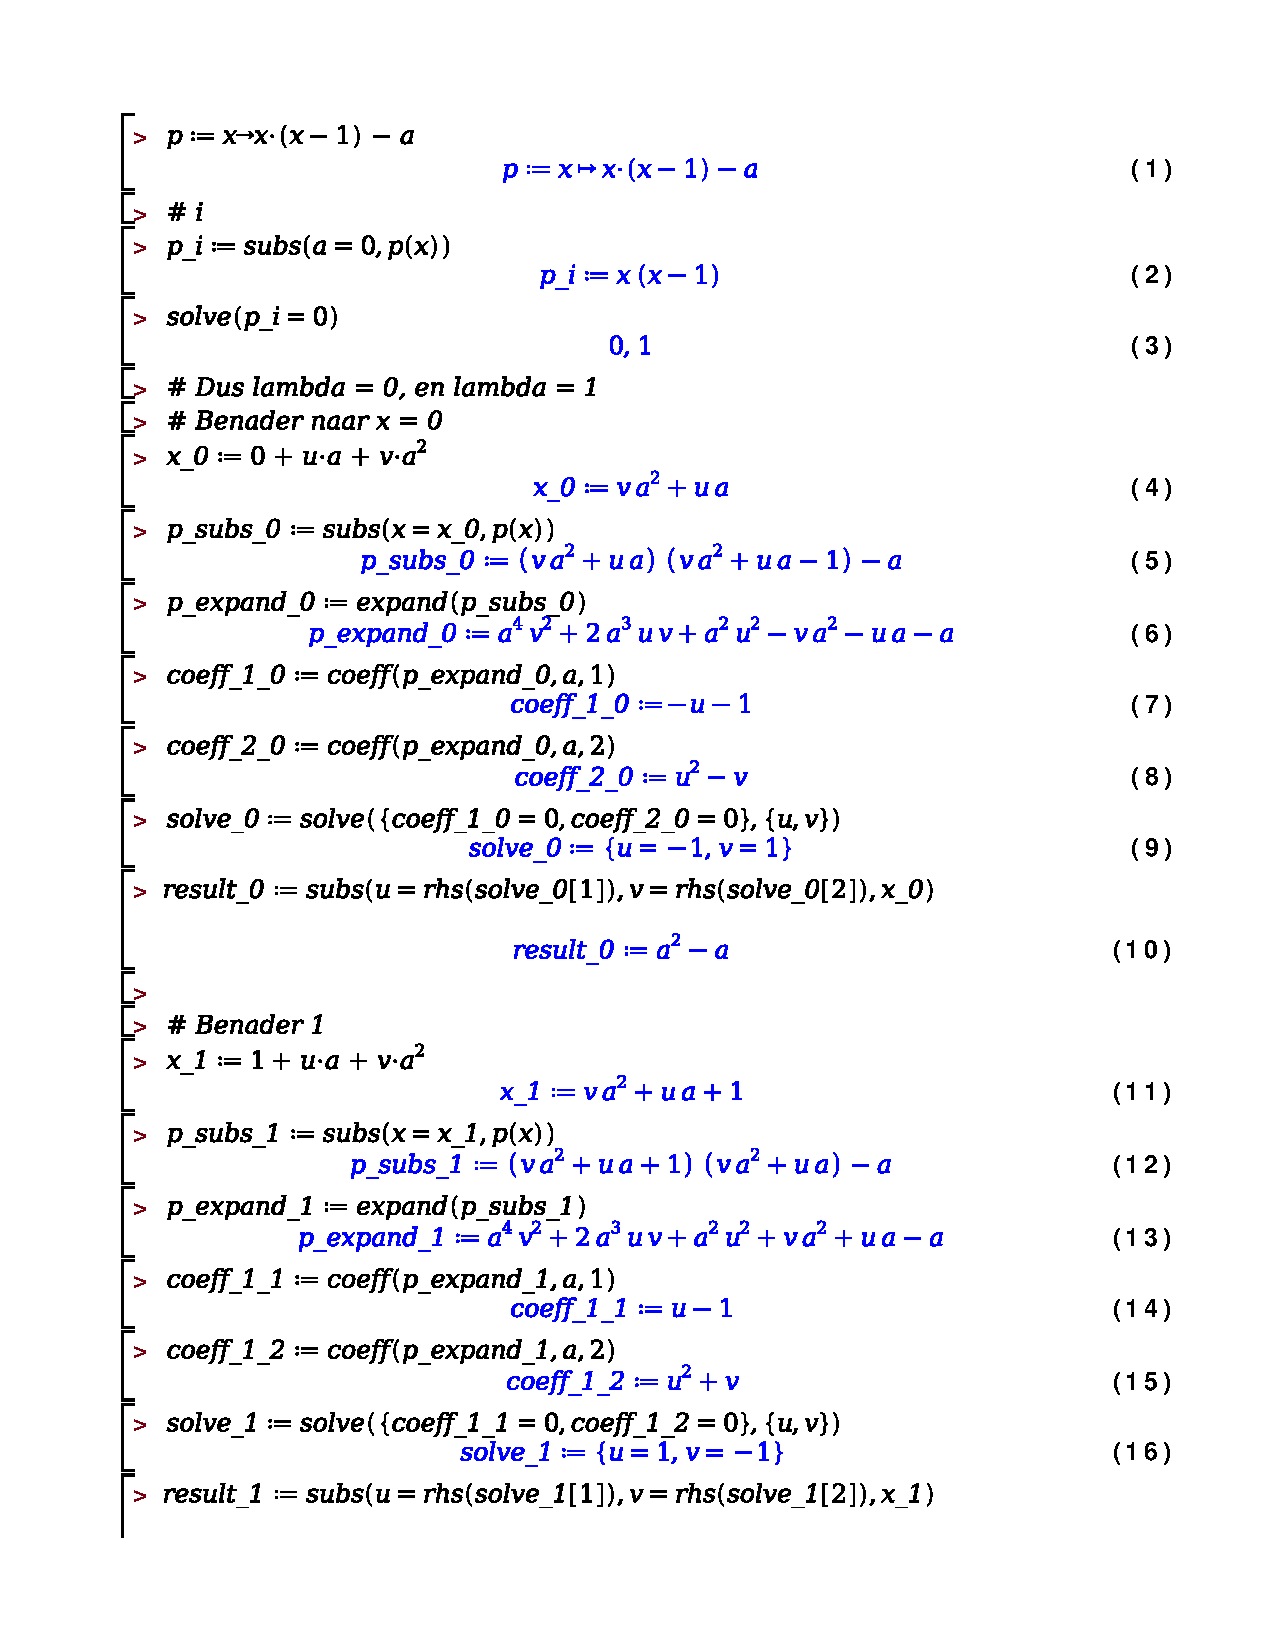
\includegraphics[width=0.8\textwidth]{./exercises/wc_1_ex_1.pdf}
	\caption{Exercise 1}
\end{figure}

\begin{figure}[!htbp]
	\centering
	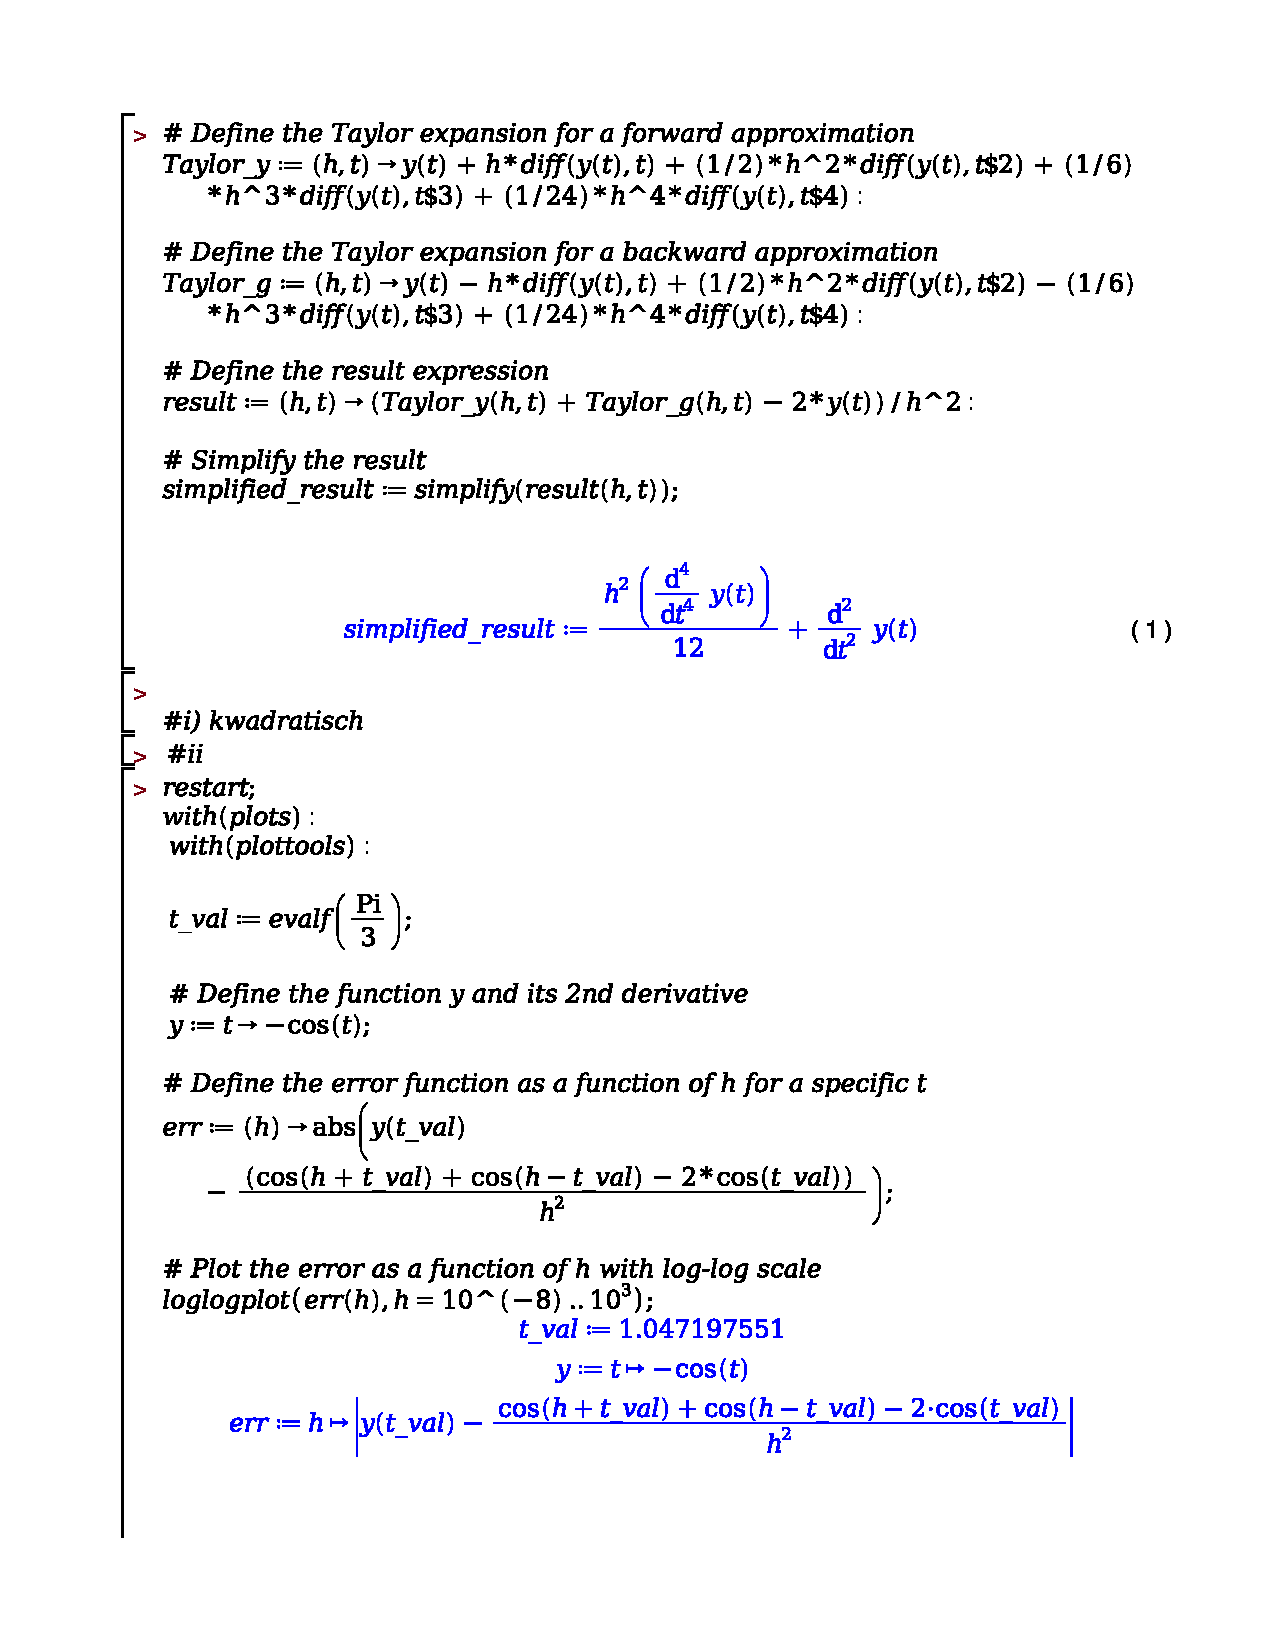
\includegraphics[width=0.8\textwidth]{./exercises/wc_1_ex_2.pdf}
	\caption{Exercise 2}
\end{figure}

\begin{figure}[!htbp]
	\centering
	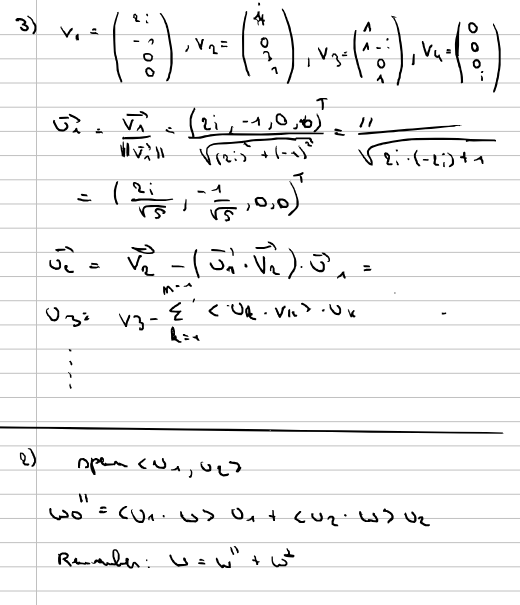
\includegraphics[width=0.8\textwidth]{images/wc1_a3.png}
	\caption{Exercise 3}
\end{figure}



\begin{figure}[!htbp]
	\centering
	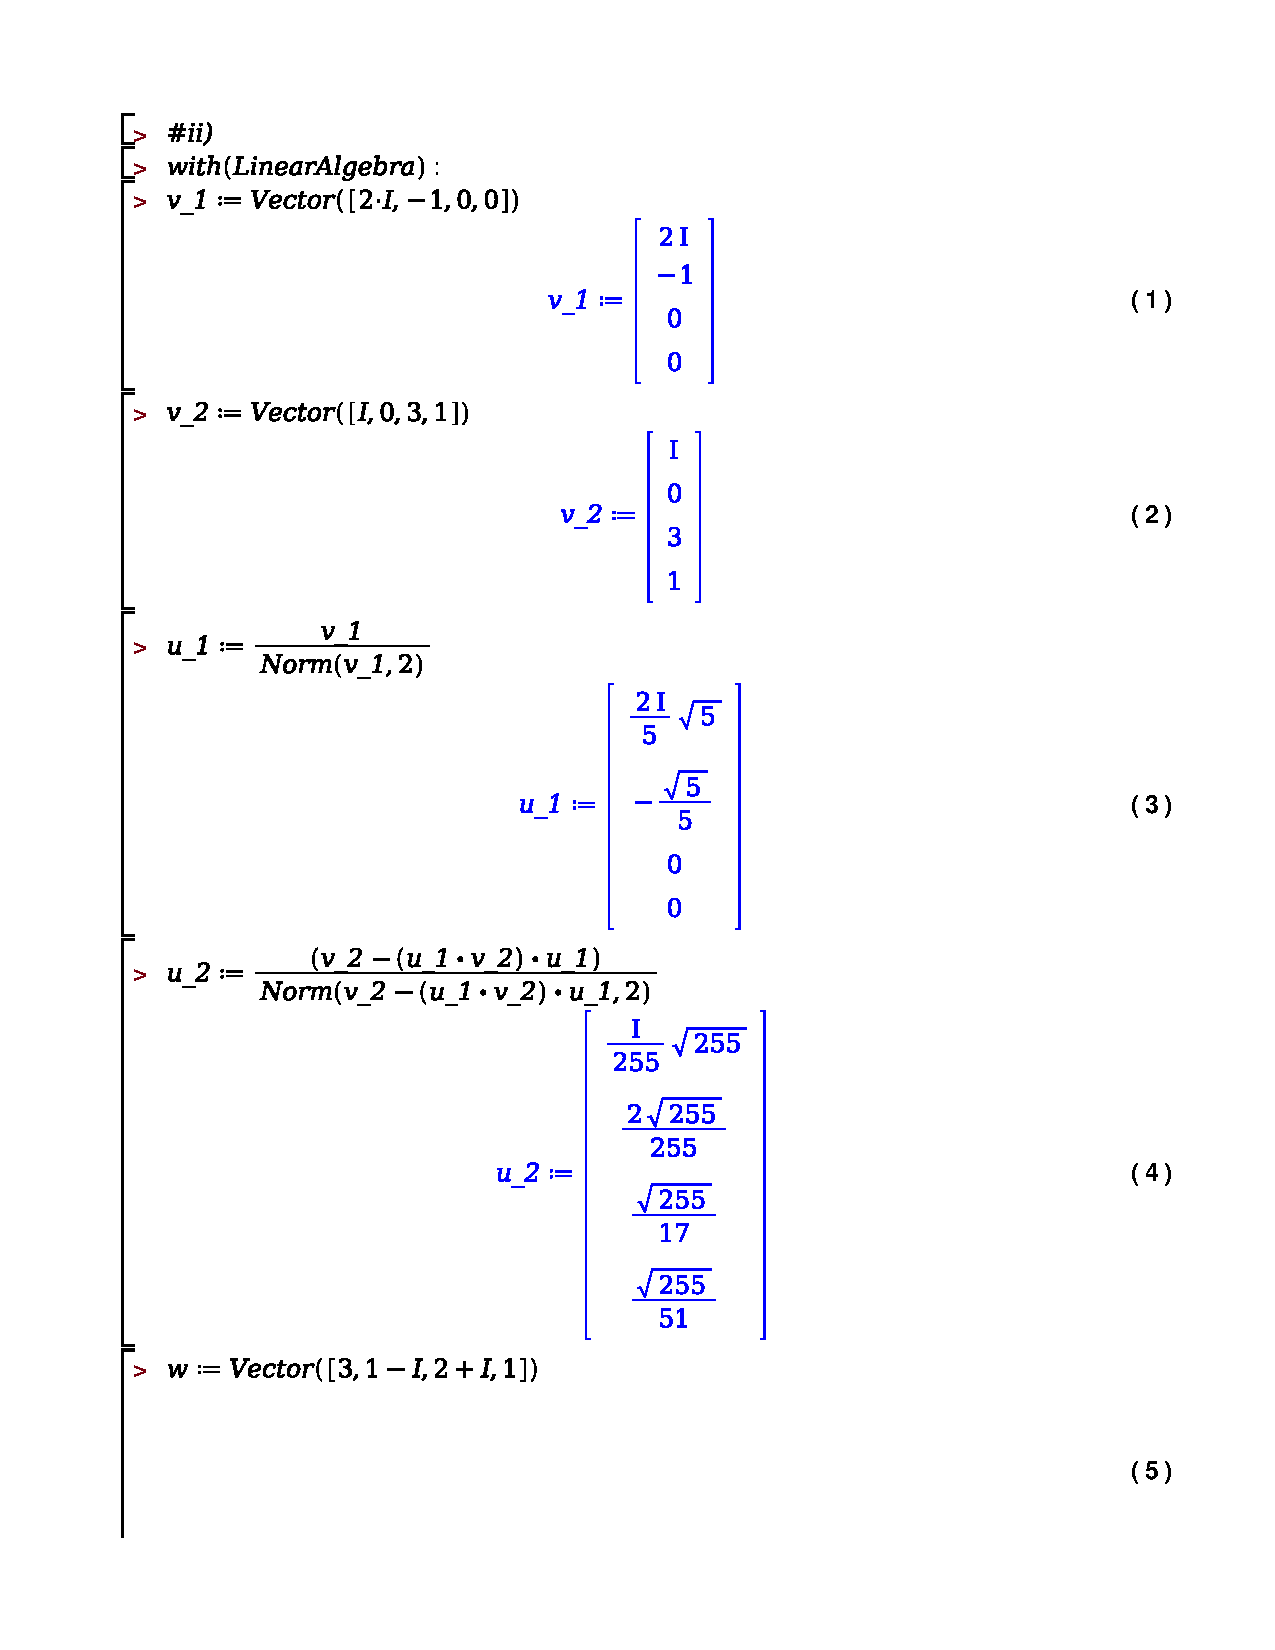
\includegraphics[width=0.8\textwidth]{./exercises/wc_1_ex_3.pdf}
	\caption{Exercise 3}
\end{figure}



\newpage
\subsection*{Bord 1}

\begin{figure}[!htbp]
	\centering
	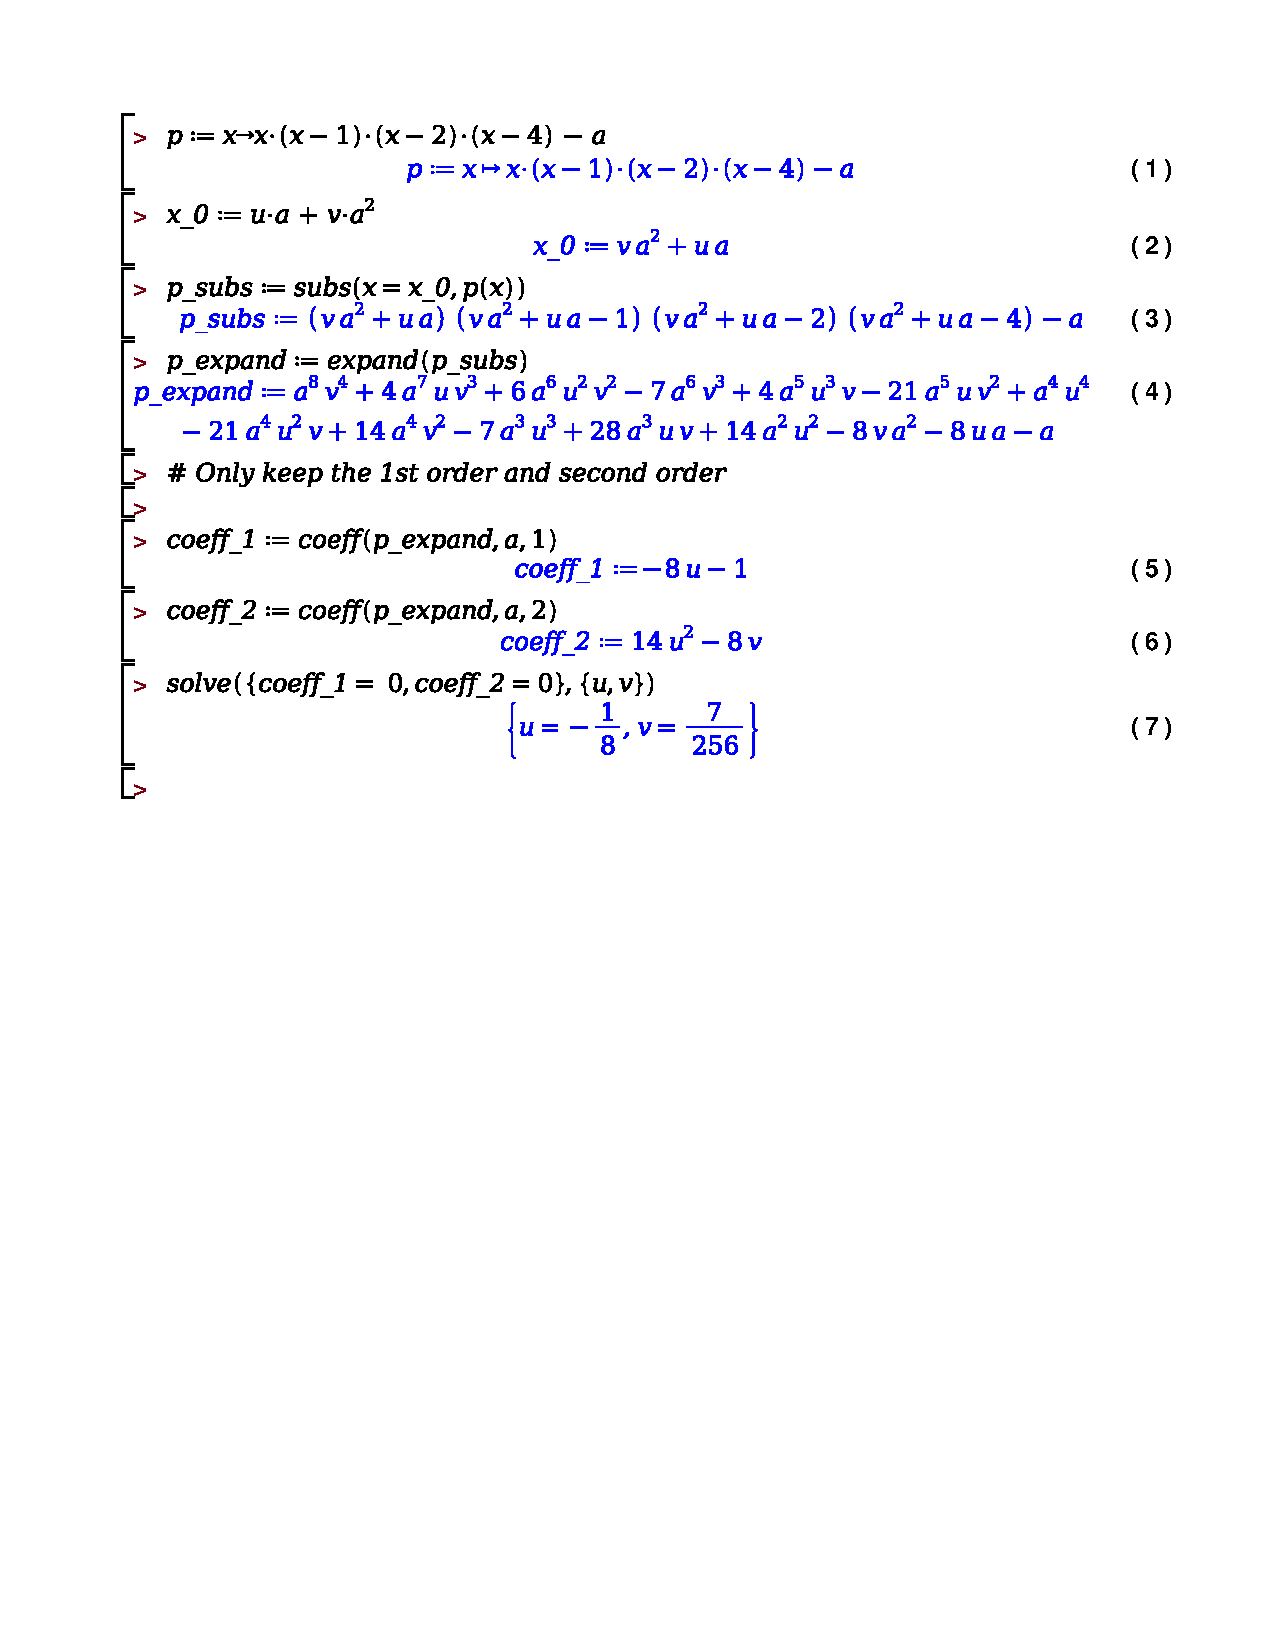
\includegraphics[width=0.8\textwidth]{./exercises/bordles_1.pdf}
	\caption{Exercise 1}
\end{figure}

\begin{figure}[!htbp]
	\centering
	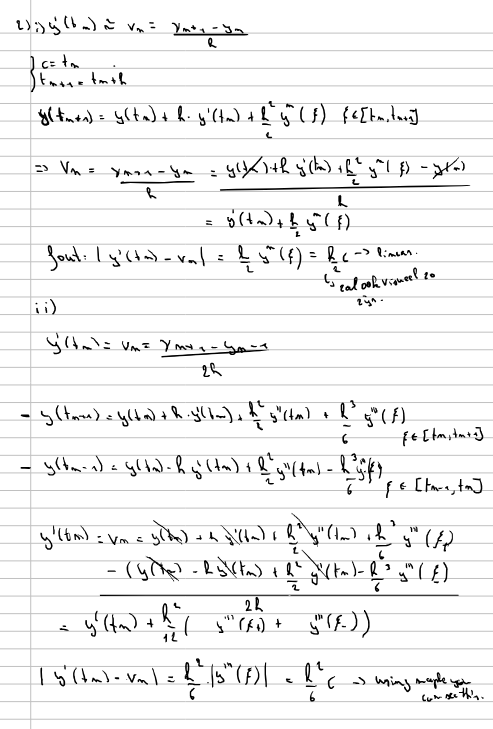
\includegraphics[width=0.8\textwidth]{images/ex_2_a.png}
	\caption{Exercise 2}
\end{figure}

\begin{figure}[!htbp]
	\centering
	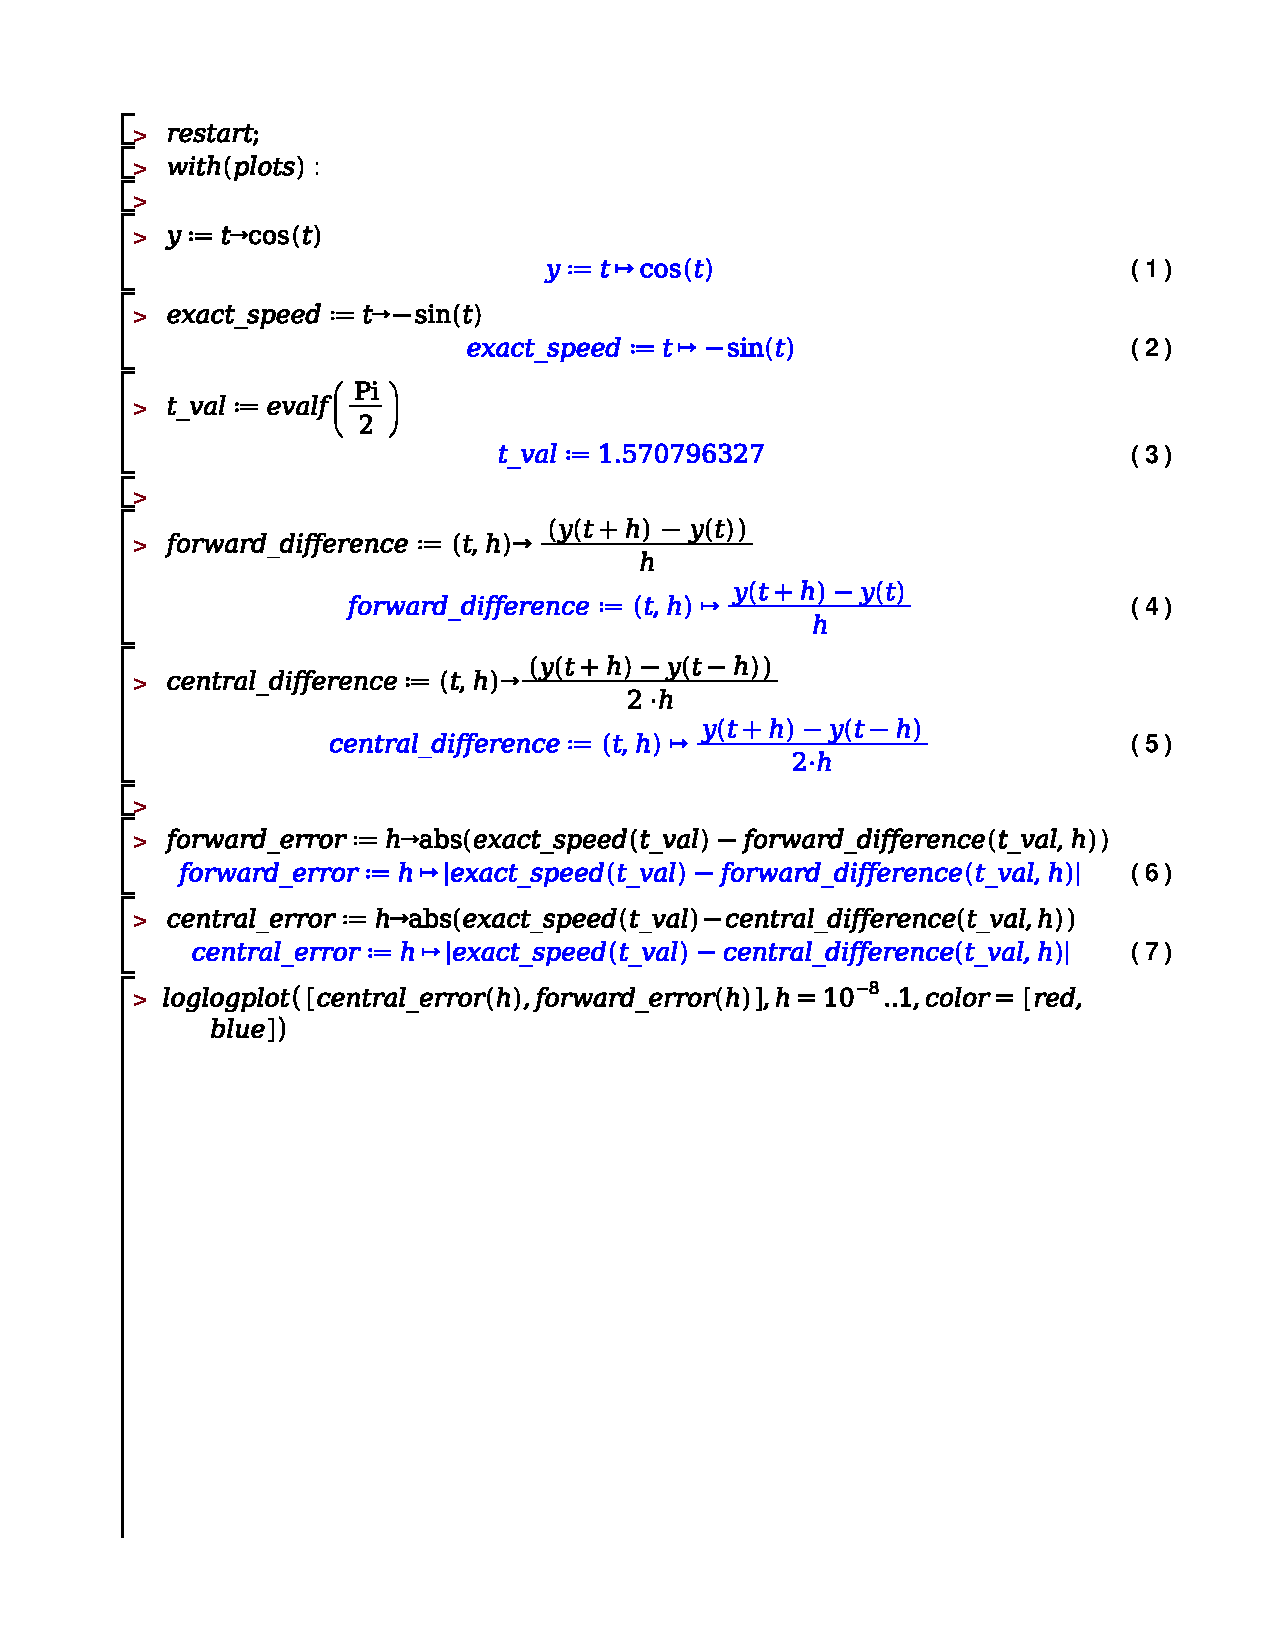
\includegraphics[width=0.8\textwidth]{./exercises/bordles_1_ex_2.pdf}
	\caption{Exercise 2 part 2 Maple}
\end{figure}

\begin{figure}[!htbp]
	\centering
	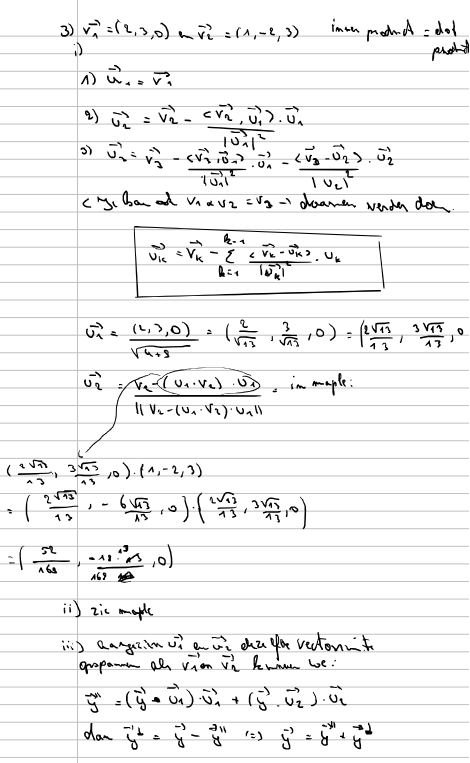
\includegraphics[width=\textwidth]{images/pl_1_answer_3.png}
	\caption{Exercise 3}
\end{figure}

\begin{figure}[!htbp]
	\centering
	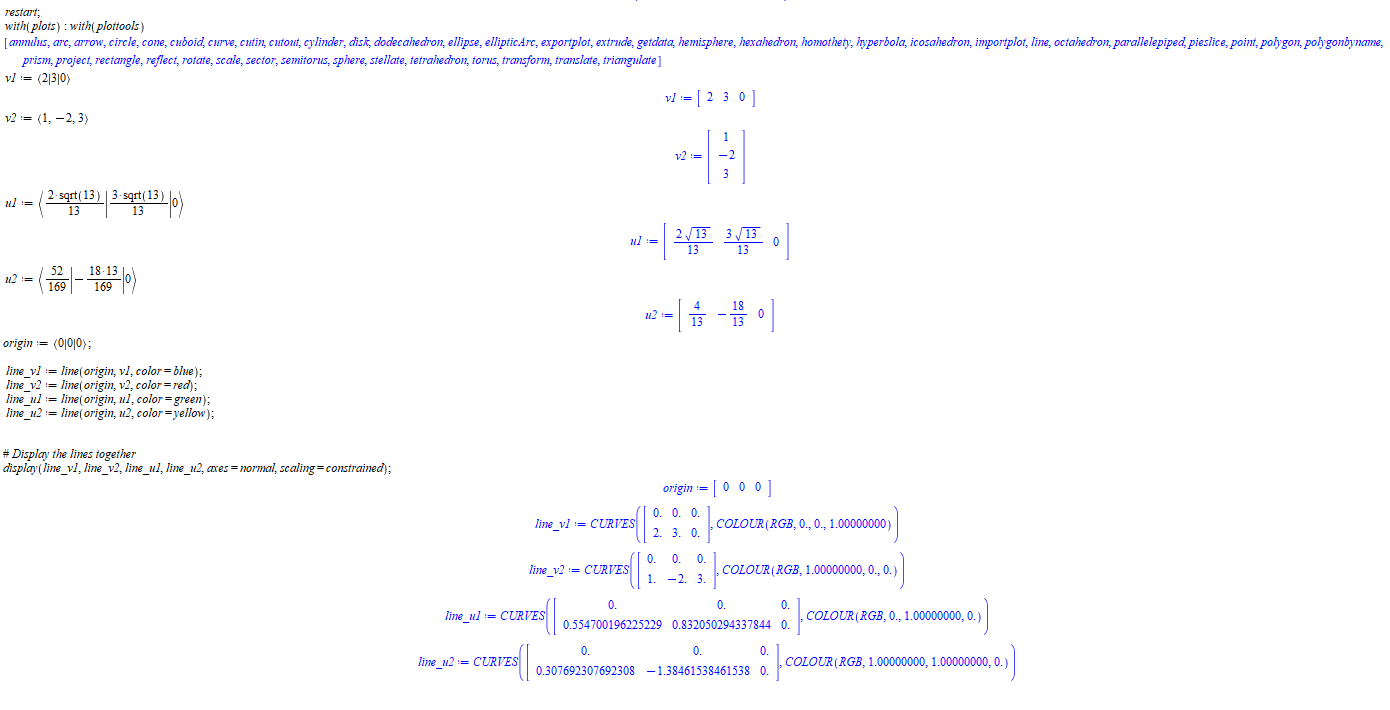
\includegraphics[width=\textwidth]{images/plot_2.png}
	\caption{Exercise 3 - plot }
\end{figure}

\begin{figure}[!htbp]
	\centering
	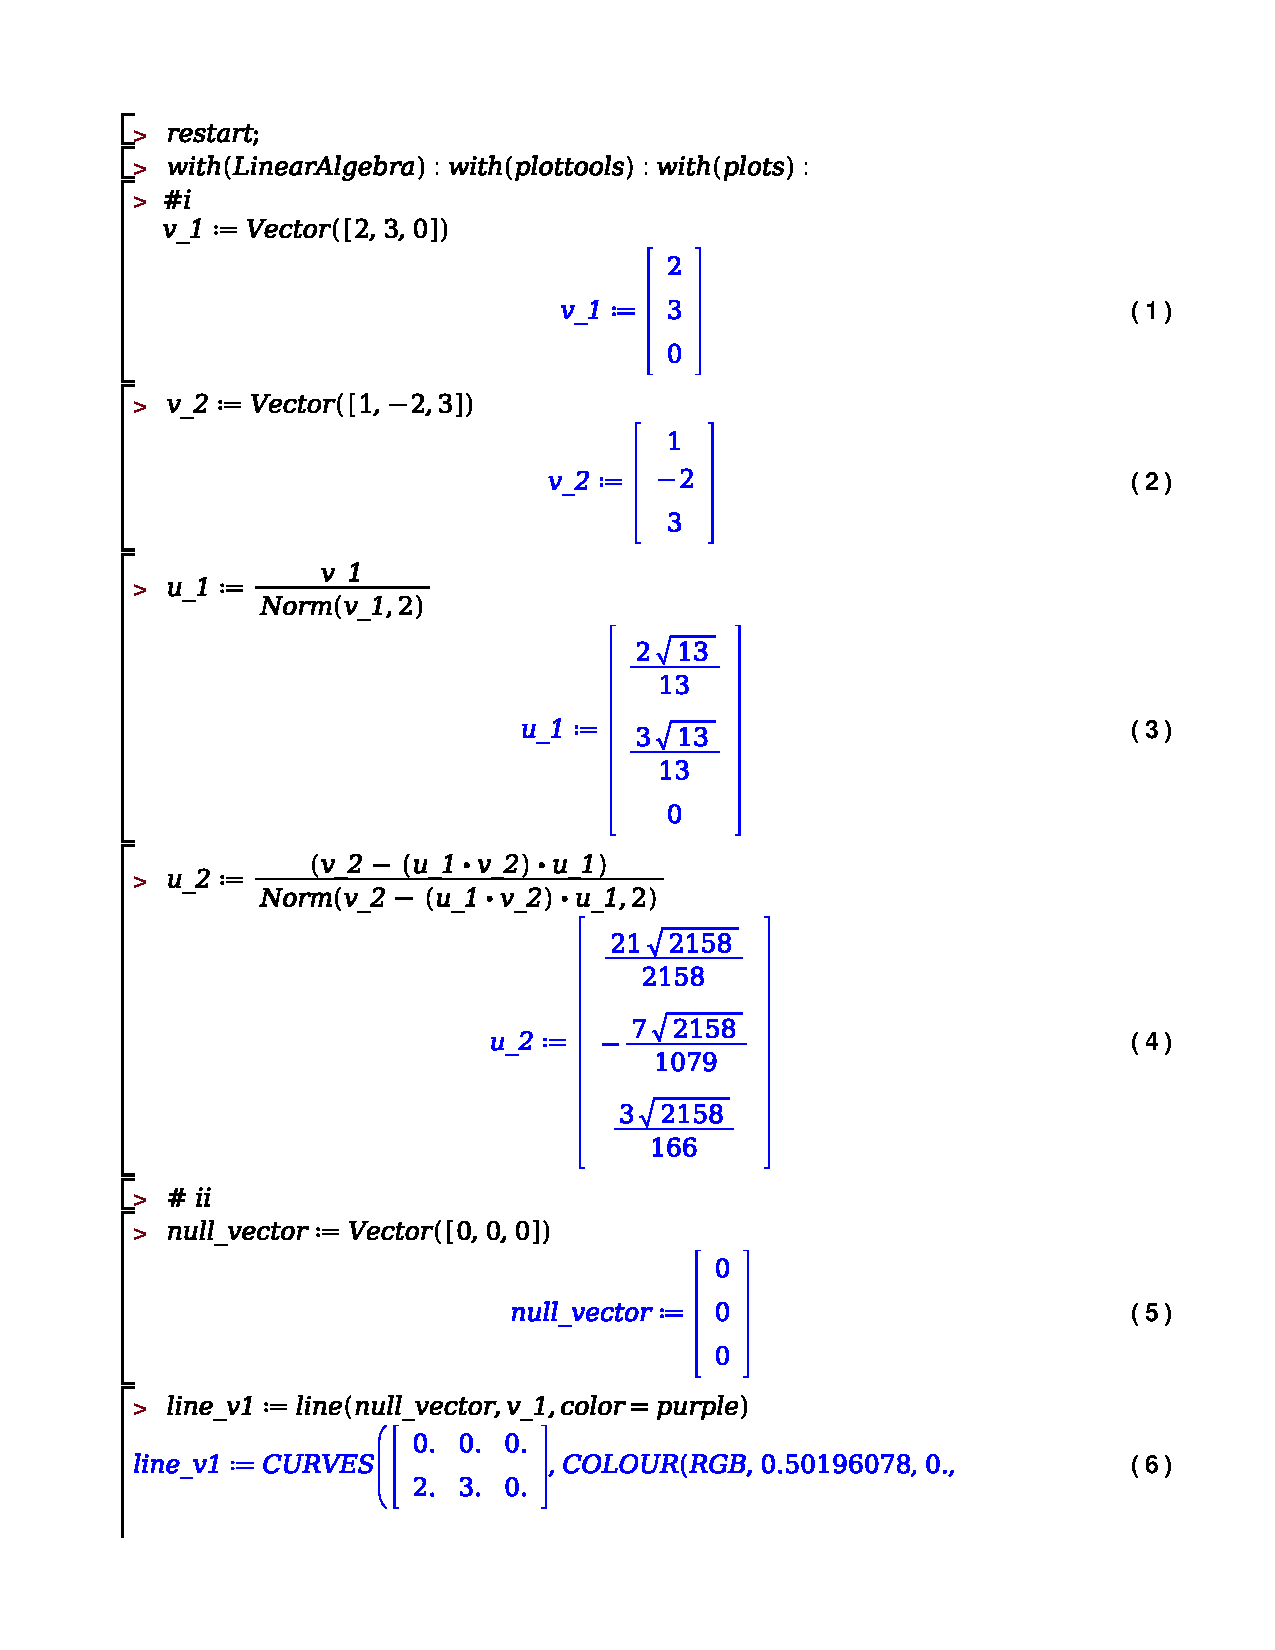
\includegraphics[width=\textwidth]{./exercises/bordles_1_ex_3.pdf}
	\caption{Exercise 3}
\end{figure}






\end{document}

\end{document}
\end{document}
